\documentclass[sn-mathphys,pdflatex,iicol]{sn-jnl}% Math and Physical Sciences Reference Style

%%%% Standard Packages
\usepackage{polyglossia} % Must come before biblatex

\usepackage{bm}
\usepackage{csquotes}
\usepackage{fontspec}
\usepackage{hyperref}
%\usepackage{lua-visual-debug}
\usepackage{tabularx}
%%%%

\jyear{2022}

%% as per the requirement new theorem styles can be included as shown below
%%\theoremstyle{thmstyleone}%
%%\newtheorem{theorem}{Theorem}[section]% meant for sectionwise numbers
%% optional argument [theorem] produces theorem numbering sequence instead of independent numbers for Proposition
%%\newtheorem{proposition}[theorem]{Proposition}%
%%\newtheorem{proposition}{Proposition}% to get separate numbers for theorem and proposition etc.

%%\theoremstyle{thmstyletwo}%
%%\newtheorem{example}{Example}%
%%\newtheorem{remark}{Remark}%

%%\theoremstyle{thmstylethree}%
%%\newtheorem{definition}{Definition}%

\raggedbottom
%%\unnumbered% uncomment this for unnumbered level heads

\setdefaultlanguage{english}
\setotherlanguage{czech}

\hypersetup{
	pdfencoding=auto,
	unicode=true,
	bookmarksopen=true,
	bookmarksopenlevel=3
}

\newcommand{\name}[1]{\textit{#1}}
\newcommand{\mathfield}{\ensuremath{\mathbb}}
\newcommand{\mathmat}{\ensuremath{\mathbf}}
\newcommand{\mathset}{\ensuremath{\mathbb}}
\newcommand{\mathspace}{\ensuremath{\mathcal}}
\newcommand{\mathvec}{\ensuremath{\bm}}

\newcounter{enumroman}
\newenvironment{romanitems}{\begin{list}{\bfseries(\roman{enumroman})\hfill}{\usecounter{enumroman}\setlength{\labelwidth}{\leftmargin}\addtolength{\labelwidth}{-1\labelsep}\topsep=0mm plus 2pt\itemsep=0mm\parsep=0mm plus 2pt\itemindent=0mm}}{\end{list}}

\DeclareMathOperator*{\argmin}{arg\,min}
\DeclareMathOperator*{\argmax}{arg\,max}


\begin{document}

\copyrightyear{2022}
\copyrightclause{Use permitted under Creative Commons License Attribution 4.0 International (CC BY 4.0).}

\conference{Data and Model Quality for Mining and Learning with Graphs: Methods and Open Challenges
@ECML-PKDD 2022, September 23, 2022, Grenoble, France}

\title{Balancing performance and complexity in hierarchical coarsening of graphs}
\author[1,2]{Marek Dědič}[orcid=0000-0003-1021-8428,email=marek@dedic.eu,url=https://dedic.eu]
\cormark[1]
\author[2]{Lukáš Bajer}
\author[2]{Jakub Repický}
\author[2]{Pavel Procházka}
\author[3]{Martin Holeňa}

\address[1]{Czech Technical University in Prague, Břehová 7, Prague, Czech Republic}
\address[2]{Cisco Systems, Inc., Karlovo náměstı́ 10, Prague, Czech Republic}
\address[3]{Institute of Computer Science, Czech Academy of Sciences, Pod vodárenskou věží 2, Prague, Czech Republic}

\cortext[1]{Corresponding author.}

\abstract{
Graph based models are used for tasks with increasing size and computational demands. We present a method for studying graph properties from the point of view of a downstream task. This method allows a user to precisely select the resolution at which the graph in question should be coarsened. Our method builds on an existing algorithm for pretraining on coarser graphs, HARP. We extend both main parts of the algorithm in order to observe the effect of graph coarsening to model quality on a fine level. We present a general framework for graph coarsenings, allowing is to cover, apart from HARP, two alternative algorithms based on graph diffusion convolution and evolutionary algorithms. Additionally, we present a novel way for refining the reduced graph in a targeted way based on the confidence of downstream classification for particular nodes. Together, these enhancements provide sufficient detail where needed, while collapsing structures where per-node information is not necessary for high model performance.
Hence, the method provides a general meta-model for enhancing graph embedding models such as node2vec. We apply it to several datasets, compare the considered coarsenings on them and discuss the differing behaviour on each of them in the context of their properties.
}

%%================================%%
%% Sample for structured abstract %%
%%================================%%

% \abstract{\textbf{Purpose:} The abstract serves both as a general introduction to the topic and as a brief, non-technical summary of the main results and their implications. The abstract must not include subheadings (unless expressly permitted in the journal's Instructions to Authors), equations or citations. As a guide the abstract should not exceed 200 words. Most journals do not set a hard limit however authors are advised to check the author instructions for the journal they are submitting to.
%
% \textbf{Methods:} The abstract serves both as a general introduction to the topic and as a brief, non-technical summary of the main results and their implications. The abstract must not include subheadings (unless expressly permitted in the journal's Instructions to Authors), equations or citations. As a guide the abstract should not exceed 200 words. Most journals do not set a hard limit however authors are advised to check the author instructions for the journal they are submitting to.
%
% \textbf{Results:} The abstract serves both as a general introduction to the topic and as a brief, non-technical summary of the main results and their implications. The abstract must not include subheadings (unless expressly permitted in the journal's Instructions to Authors), equations or citations. As a guide the abstract should not exceed 200 words. Most journals do not set a hard limit however authors are advised to check the author instructions for the journal they are submitting to.
%
% \textbf{Conclusion:} The abstract serves both as a general introduction to the topic and as a brief, non-technical summary of the main results and their implications. The abstract must not include subheadings (unless expressly permitted in the journal's Instructions to Authors), equations or citations. As a guide the abstract should not exceed 200 words. Most journals do not set a hard limit however authors are advised to check the author instructions for the journal they are submitting to.}

\keywords{
  Graph representation learning,
  Graph coarsening,
  Graph diffusion,
  Graph homophily,
  Performance-complexity trade-off,
  HARP
}


\maketitle

\todo{Abstract}
\todo{Keywords}
\section{Introduction}
Across a wide variety of applications and domains, graphs emerge as a domain-independent and ubiquitous way of organizing data. Consequently, machine learning on graphs has, in recent years, seen an explosion in popularity, breadth and depth of both research and applications. While there have been significant advances in algorithms for learning from graph data \cite{defferrard_convolutional_2016, kipf_semi-supervised_2017, li_deepergcn_2020}, the structure of the underlying data has, until recent works \cite{gasteiger_diffusion_2019, topping_understanding_2021, velickovic_geometric_2021, chamberlain_grand_2021}, received much less attention. In this work, we aim to take a closer look at the importance of the individual nodes and neighbourhoods that form a graph from the point of view of downstream tasks.

Typically, an application of machine learning to graphs has two phases: representation learning, which maps the graph into a Euclidean space, and a downstream task, such as classification, regression, or clustering. The first phase has very high computational demands, which can be substantially decreased with graph coarsening. However, it is known that there is an interplay between coarsening and the quality of embedding \cite{akyildiz_understanding_2020, makarov_survey_2021}, which in turn entails an interplay between coarsening and the quality of the downstream task.

Our work builds on the HARP \cite{chen_harp_2018} method for pretraining on coarsened graphs. In HARP, a graph is repeatedly coarsened and the coarser graphs are then used in reverse order (from coarsest to finest) to pre-train a graph representation learning algorithm. While HARP itself works with and modifies the graph structure, this is not the main interest of its authors, who focus more on the obtained representation of the original graph. In our work, we aim to leverage such a graph coarsening approach to study the properties of graphs and graph embedding models from the point of view of the graph structures getting coarsened with the additional benefit of decreasing computational requirements. We modify and generalize the HARP framework to closely study the relationship between graph coarsenings and graph quality in terms of the performance of a downstream task. In our case, we chose transductive node classification as the ultimate task, however, the presented algorithms are general graph representation learners that can be utilized for a wide variety of tasks.

\todo[inline]{Relation to ITAT paper?}

The main contributions of this work are the general framework for graph coarsening and extensions of the HARP algorithm. We extend both main parts of the algorithm in order to observe the effect of graph coarsening to model quality on a fine level. We present two alternative graph coarsening schemes based on graph diffusion convolution and evolutionary algorithms. Additionally, we present a novel way for un-coarsening the reduced graph in a targeted way based on the confidence of downstream classification for particular nodes.

In the next section, related work and its relationship to this work are discussed. Following that, in Section \ref{sec:harp-framework}, HARP, the method our work builds on, is presented, together with our extension of it into a general framework for graph coarsening. Section \ref{sec:our-method} is the core of this work, presenting first our extension of the prolongation step, as well as our proposed alternative graph coarsening schemes. Finally, these proposals are experimentally verified and compared in Section \ref{sec:experimental-evaluation}.

\section{HARP}\label{sec:harp}

\subsection{Method overview}

\subsection{Graph coarsening}\label{sec:graph-coarsening}

\subsection{Embedding prolongation}
In each coarsening step, an embedding of the graph \( G_i \) is trained by one of the embedding algorithms. To continue training with a finer graph, this embedding \( \Phi_i: V \left( G_i \right) \to \mathfield{R}^d \) needs to be \textit{prolonged} to create the finer embedding \( \Phi_{i - 1}: V \left( G_{i - 1} \right) \to \mathfield{R}^d \). To achieve this, the representation of a node in the graph \( G_i \) is copied for each of the nodes in \( G_{i - 1} \) it was created from (by the graph collapsing algorithm). That is,
\[ \Phi_{i - 1} \left( u \right) = \Phi_i \left( \psi_i \left( u \right) \right)\text{.} \]
This is then taken as the starting point for the next training phase.

\section{Partially injective homomorphism}

In \cite{schulz_mining_2019}, the authors present the notion of \textbf{partially injective homomorphisms} as a bridge between the comparatively weak concept of a homomorphism and the much stronger concept of an injective homomorphism (i.e., a subgraph isomorphism). This section presents these concepts and explores some of their properties. In Section \ref{sec:harp-as-pihom}, graph homomorphisms are then used as a general framework for graph coarsening.

A \textbf{graph homomorphism} between graphs \( G \) and \( H \) is a mapping \( \varphi: V \left( G \right) \to V \left( H \right) \) that preserves edges, thus
\[ \left( u, v \right) \in E \left( G \right) \implies \left( \varphi \left( u \right), \varphi \left( v \right) \right) \in E \left( H \right) \text{.} \]
A homomorphism is \textbf{injective} iff \( \forall u, v \in V \left( G \right) \quad \varphi \left( u \right) = \varphi \left( v \right) \implies u = v \text{.} \)
Finally, a homomorphism is \textbf{partially injective} iff
\( \forall \left( u, v \right) \in \mathcal{C} \quad \varphi \left( u \right) = \varphi \left( v \right) \implies u = v \)
for some \( \mathcal{C} \subseteq \left( V \left( G \right) \right)^2 \setminus E \left( G \right) \), that is, \( \mathcal{C} \) is a set of \textit{non-edges} of the graph \( G \).
Observe that for any \( \left( u, v \right) \in E \left( G \right) \) the condition holds in general per the definition of a homomorphism on a graph without loops, which justifies the limitation of \( \mathcal{C} \) to non-edges of the graph.

For given graphs \( G \) and \( H \), let \( \mathcal{L} \) denote the finite set of all partially injective homomorphisms between them. Let a particular partially injective homomorphism described by \( \mathcal{C} \) be denoted as \( \mathrm{PIHom} \left( G, H, \mathcal{C} \right) \). \( \mathcal{L} \) has a natural partial order \( \preceq \) where \( \mathrm{PIHom} \left( G, H, \mathcal{C}_1 \right) \preceq \mathrm{PIHom} \left( G, H, \mathcal{C}_2 \right) \) iff \( \mathcal{C}_1 \subseteq \mathcal{C}_2 \) and forms a lattice with order \( \preceq \). The minimum of this lattice \( \mathrm{PIHom} \left( G, H, \emptyset \right) \) corresponds to an ordinary homomorphism while the maximum \(\mathrm{PIHom} \left( G, H, \left( V \left( G \right) \right)^2 \setminus E \left( G \right) \right) \) corresponds to an injective homomorphism.

\section{HARP and partially injective homomorphisms}\label{sec:harp-as-pihom}

The connection between HARP and partially injective homomorphisms is a theoretical, yet useful one. If the HARP coarsenings could be restricted to partially injective homomorphisms or their compositions, general coarsenings could be learned for each task. In Section \ref{sec:harp-vs-pihom} we explore whether this restriction limits the performance of HARP.

When both the edge and star collapsing algorithms are used, the mapping \( \psi_i \) introduced in \ref{sec:graph-coarsening} is \textbf{not} a homomorphism nor a combination of homomorphisms due to its not meeting the injectivity condition on edges. However, it is met for the complementary graph (graph where edges are swapped with non-edges). For the complementary graph, the star collapsing algorithm is not a homomorphism, however, it can be replaced by homomorphisms that also collapses stars. We propose a coarsening that merges a hub node with half of its neighbours. Because merging a node with its neighbour only collapses an edge, this coarsening scheme is a composition of partially injective homomorphisms on the complementary graph. Such a model is studied in Section \ref{sec:harp-vs-pihom}.

This theoretical connection gives a way of constructing more general graph coarsenings by setting a constraint on such relations and finding the maximum of a subset of \( \mathcal{L} \) that satisfies such a constraint. The authors of \cite{schulz_mining_2019} present a way of effectively (in polynomial time for bounded tree-width graphs) searching for such maximally constrained homomorphisms.

\section{HARP and the performance-complexity trade-off}\label{sec:performance-vs-complexity}

Graph-based methods such as node2vec typically have a large number of parameters - on the widely used OGBN-ArXiv dataset (see \cite{hu_open_2021}), the SOTA node2vec model has over 21 million parameters. At the same time, recent works have started to focus more heavily on simpler methods as a competitive alternative to heavy-weight ones (see \cite{frasca_sign_2020,huang_combining_2020,salha_keep_2019,zhang_eigen-gnn_2020}). As the authors of \cite{chen_harp_2018} observed, HARP improves the performance of models when fewer labelled data are available. The proposed lower complexity models based on HARP could also improve performance in a setting where only low fidelity data are available for large parts of the graph. Coarser models could be trained on them, with a subsequent training of finer models using only a limited sample of high fidelity data.

As a core principle of HARP, lower level representations of the task are generated and a model is learnt on them. How good these models are remains in question. In order to test this, several models were compared. Each model \( M_i \) was trained on graphs \( G_L, \dots, G_i \) as with HARP, then the embeddings were prolonged on graphs \( G_{i-1}, \dots, G_0 \) without training. On \( G_0 \), the models were then trained as they would be in an ordinary node2vec setup. With this schema, \( L \) models are obtained, each trained on graphs of different granularity. As the coarsers graphs are much smaller in size, the pretraining is much more efficient to compute that training on the original graph. To examine the performance-complexity trade-off of HARP, the trade-off between decreasing predictive accuracy and decreasing amount of training data was evaluated.

\section{Experimental evaluation}\label{sec:experiments}

The experiments proposed in the previous sections were run on the OGBN-ArXiv dataset (see \cite{hu_open_2021}) with node2vec as the underlying graph learning algorithm. The experiments build upon the SOTA node2vec implementation for this dataset.

\subsection{Experiment setup}

The configurations of both the node2vec and the MLP models are taken from the PyTorch Geometric implementation of node2vec on the ogbn-arxiv dataset (a dataset of 169 343 computer science arXiv papers, see \cite{paszke_pytorch_2019}), which was also used for the experiments. The node2vec model generated an embedding into \( \mathfield{R}^{128} \) from \( 10 \) random walks of length \( 80 \) for each node with a context window size of \( 20 \). The optimizer ADAM \cite{kingma_adam:_2017} was used with a learning rate of \( 0.01 \) and batches of \( 256 \) samples. The MLP classifier using the embeddings featured \( 3 \) linear layers of \( 256 \) neurons with batch normalization after each layer. Finally, a linear layer was used for the class prediction. ADAM with a learning rate of \( 0.01 \) and a dropout rate of \( 0.5 \) was used for \( 200 \) epochs of training with the cross-entropy loss function. The experiments were implemented using PyTorch\footnote{https://pytorch.org/} and PyTorch Geometric \cite{paszke_pytorch_2019}.

\subsection{Effect of HARP pretraining}

\begin{table}
  \caption{Size of the graphs generated at different coarsening levels.}
  \label{tab:graph-sizes}
  \begin{tabular}{lrr}
    \toprule
    Graph     & \# of nodes & \# of edges \\
    \midrule
    \( G_0 \) & 169 343     & 2 315 598   \\
    \( G_1 \) & 67 496      & 1 886 875   \\
    \( G_2 \) & 29 408      & 1 558 368   \\
    \( G_3 \) & 15 039      & 1 252 276   \\
    \( G_4 \) & 9 273       & 815 493     \\
    \( G_5 \) & 6 768       & 433 795     \\
    \( G_6 \) & 5 607       & 197 876     \\
    \( G_7 \) & 4 994       & 86 307      \\
    \( G_8 \) & 4 655       & 42 441      \\
    \( G_9 \) & 4 404       & 29 167      \\
    \bottomrule
  \end{tabular}
\end{table}

\begin{figure}
  \centering
  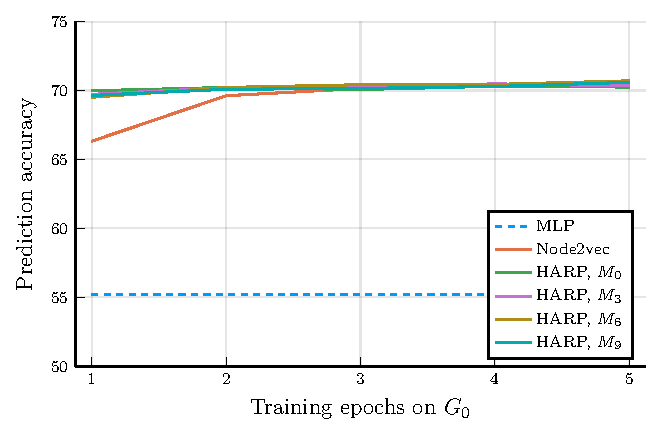
\includegraphics[width=\linewidth]{images/steps_accur/steps_accur.pdf}
  \caption{Performance over epochs of models pretrained on different coarsening levels.}
  \label{fig:steps-accuracy}
\end{figure}

To asses the effect of HARP as a pretraining, the main question is how does HARP pretraining change the behaviour of the node2vec training? To this end, 10 different models \( M_0, \dots, M_9 \) as defined in Section \ref{sec:performance-vs-complexity} were trained. The sizes of the respective graphs \( G_0, \dots, G_9 \) are denoted in Table \ref{tab:graph-sizes}.

Figure \ref{fig:steps-accuracy} compares the accuracy of several models over learning epochs on the original graph \( G_0 \). An MLP using just dataset features and an ordinary node2vec model are provided as a reference. The models \( M_0, \dots, M_9 \) are then compared.

As can be seen, there is no noticeable difference in the performance of a pretrained node2vec in comparison to an ordinary one when it comes to performance after 4 or more training epochs. Our explanation is that the configuration used for node2vec training already samples large parts of the graph thanks to a relatively high number of long random walks. There is, however, a noticeable improvement in the performance of models when only very few training epochs are available.

\subsection{Feasibility of partially injective transformations}\label{sec:harp-vs-pihom}

\begin{figure}
  \centering
  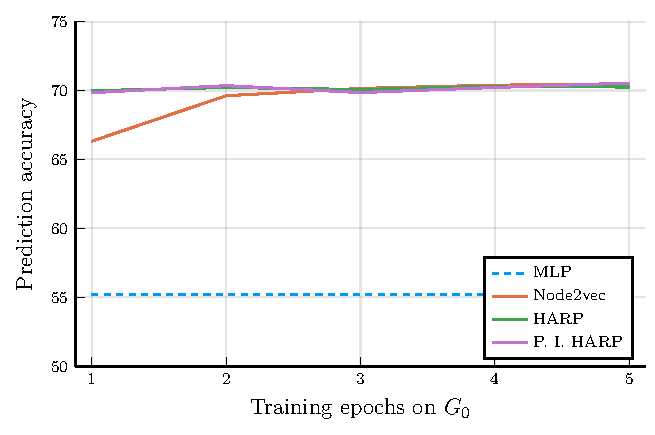
\includegraphics[width=\linewidth]{images/pihom_comparison/pihom_comparison.pdf}
  \caption{Standard HARP compared to the version built on partially injective homomorphisms.}
  \label{fig:HARP-vs-PIHom}
\end{figure}

In order to test the feasibility of HARP-like algorithms based purely on partially injective homomorphisms, ordinary HARP is compared to one with the coarsening proposed in Section \ref{sec:harp-as-pihom}. Figure \ref{fig:HARP-vs-PIHom} shows the performance of such a model compared to ordinary HARP, node2vec and purely feature-based MLP classifier. As can be seen, there is no meaningful difference between the two models.

\section{Future work}

In this work-in-progress, two properties of graph-based models are studied. While these properties seem to be unconnected at first, they are both highly relevant to the future progress of our work. The target use of these approaches is the detection of similar sub-structures in graphs of very large size. It is computationally unfeasible to use techniques such as graph convolution for extremely large graphs. With HARP, such graphs could be significantly reduced in size, enabling the use of such more computationally demanding techniques. Also, the way in which the graphs are coarsened can be specifically tailored in a way that either preserves, or collapses the subgraphs of interest. Using such tailored coarsening techniques would allow for scanning for a pre-determined structure in the graph.

The target application of this work lies in the domain of computer network security. Malware running on endpoint devices connects to remote resources, i.e. as a check for internet connectivity or a connection to a Command \& Control server. From the traffic of regular user-induced behaviour as well as malware, a connection map can be built and represented with a graph. A skilled analyst can recognize nodes and edges associated with malicious software, however, in the present time, some families of malware are either sold to multiple threat actors and set up with duplicate infrastructure or they change the infrastructure they use as a means of evading detection. Our work aims towards recognizing such duplications or changes in infrastructure previously marked as malicious by an analyst. Moreover, the methods studied could enable automatic recognition of new infrastructure employed by previously seen malware families and suggest it for manual review, thus dramatically reducing the time needed until the new infrastructure is discovered. 

\section{Conclusion}

In our work in progress, a way to merge method generality, computational efficiency and high performance was explored. HARP and partially injective homomorphisms were presented and subsequently connected as a way to, in a future work, adapt graph coarsenings to a specific task. This connection was experimentally verified not to impact prediction performance. Furthermore, the effect of HARP pretraining on learning characteristics was studied and found to reduce the need for training on fine (and therefore large) graphs, making way for a more efficient training without sacrificing performance.


\begin{acknowledgments}
  The research reported in this paper has been supported by the Czech Science Foundation (GAČR) grant 18-18080S.
\end{acknowledgments}

\bibliography{zotero}

\end{document}
